\documentclass{article} 
 \usepackage{graphicx}
 \usepackage{caption}
  \usepackage{caption}
  \usepackage[T1]{fontenc}
  
\begin{document} % > Compilar con PDFLaTeX
 
 Consideremos ahora el paralelep�pedo
 
 \begin{figure}[h!] % Ambiente 'figure'
  \centering        % imagen sin escalar
  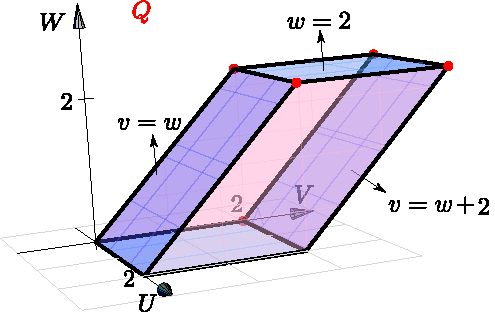
\includegraphics{images/figura3.pdf}
  \caption{Un paralelep�pedo}\label{figura3}  
 \end{figure}
 
 Ahora consideremos el s�lido $Q$...
 
 \begin{center} % Escalada a 4cm de ancho
  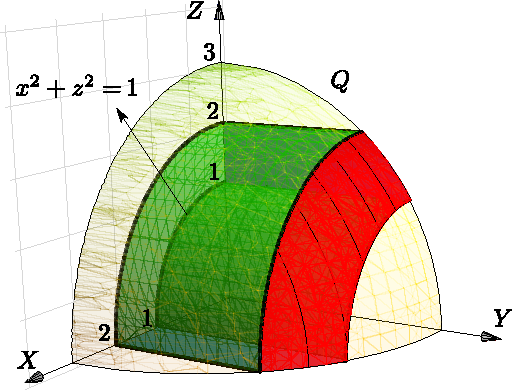
\includegraphics[width=5cm]{images/figura4.pdf}
  \captionof{figure}{S�lido $Q$}
  \label{figura3a} 
 \end{center}
 
\end{document}